\documentclass[11pt]{article}
\usepackage{hyperref}
\usepackage{natbib}
\usepackage{amsmath}
\usepackage{nicefrac}
\usepackage[usenames,dvipsnames]{xcolor}
\usepackage{graphicx}
\usepackage{footnote}
\usepackage{rotating}
\usepackage{slashbox}
\usepackage{afterpage}
\usepackage{float}
\citestyle{apj}
%%%%%%%%%%%%%%%%%%%%%%%%%%%%%%%%%%%%%%%%%%%%%%%%%%%%%%%%%%%%%%%%%%%%%%%%%%%%
%force setting figures at the top of the page:
    \makeatletter
    \setlength{\@fptop}{0pt}
    \makeatother
%%%%%%%%%%%%%%%%%%%%%%%%%%%%%%%%%%%%%%%%%%%%%%%%%%%%%%%%%%%%%%%%%%%%%%%%%%%%
%  personal abbreviations and macros
%    the following package contains macros used in this document:
%\input econfmacros.tex
%%%%%%%%%%%%%%%%%%%%%%%%%%%%%%%%%%%%%%%%%%%%%%%%%%%%%%%%%%%%%%%%%%%%%%%%%%%
\textwidth=6.9in  \textheight=9.6in
%%  Adjust these for your printer:
\leftmargin=-5in   \topmargin=-0.8in
\hoffset = -0.95in  \voffset = 0pt
\marginparwidth = 0pt
%% preprint number data:
%\newcommand\pubnumber{Article 14 in eConf C1304143}
\newcommand\pubnumber{}
\newcommand\pubdate{\today}

%%  address and funding acknowledgement data:
\def\affiliation{Department of Physics \\
The University of Texas at Austin, TX 78712, USA; amir@physics.utexas.edu}
%\def\support{\footnote{Work supported by the Office of Science,Kingdom of the Two Sicilies, under contract OSS--32456.}}

%%%%%%%%%%%%%%%%%%%%%%%%%%%%%%%%%%%%%%%%%%%%%%%%%%%%%%%%%%%%%%%%%%%%%%%%%%%%
%   document style macros
%%%%%%%%%%%%%%%%%%%%%%%%%%%%%%%%%%%%%%%%%%%%%%%%%%%%%%%%%%%%%%%%%%%%%%%%%%%%
\def\gtrsim{\mathrel{\hbox{\rlap{\hbox{\lower4pt\hbox{$\sim$}}}\hbox{$>$}}}}
\def\lessim{\mathrel{\hbox{\rlap{\hbox{\lower4pt\hbox{$\sim$}}}\hbox{$<$}}}}
\newcommand{\ddg}{$\Delta\Delta G~$}
%\newcommand{\se}{\it seqent}
%\newcommand{\rs}{\it r4sJC}

%%%%%%%%%%%%%%%%%%%%%%%%%%%%%%%%%%%%%%%%%%%%%%%%%%%%%%%%%%%%%%%%%%%%%%%%%%%%
\def\Title#1{\begin{center} {\Large #1 } \end{center}}
\def\Author#1{\begin{center}{ \sc #1} \end{center}}
\def\Address#1{\begin{center}{ \it #1} \end{center}}
\def\andauth{\begin{center}{and} \end{center}}
\def\submit#1{\begin{center}Submitted to {\sl #1} \end{center}}
\newcommand\pubblock{\rightline{\begin{tabular}{l} \pubnumber\\
         \pubdate  \end{tabular}}}
\newenvironment{Abstract}{\begin{quotation}  }{\end{quotation}}
%\newenvironment{Presented}{\begin{quotation} \begin{center}
%             PRESENTED AT\end{center}\bigskip
%      \begin{center}\begin{large}}{\end{large}\end{center} \end{quotation}}
\def\Acknowledgements{\bigskip  \bigskip \begin{center} \begin{large}
             \bf ACKNOWLEDGEMENTS \end{large}\end{center}}

\graphicspath{{../analysis/figures/}}

\begin{document}
\begin{titlepage}
\pubblock

\vfill
\Title{Sequence Divergence as the main modulator of structure-sequence correlations}
\vfill
\Author{Amir Shahmoradi, Claus Wilke, Eleisha Jackson, ...}%\support}
\Address{\affiliation}
\vfill
\begin{Abstract}
    Over the past decade several independent works have shown that some site-specific structural properties of proteins are capable of predicting the site-specific evolutionary sequence variations. The strength and significance of these structure-evolution relations, however, appear to vary widely among different proteins, with absolute correlation strengths ranging from $0.1$ to $0.8$. In search for potential determinants of the observed variation in sequence-structure correlations, here we present the results of a comprehensive study of interrelations among more than $200$ structural and evolutionary characteristics in a dataset of 209 monomeric enzymes. We identify sequence divergence as the main determinant of the strengths of virtually all structure-evolution relationships, explaining $\sim10-30\%$ of observed variation in correlation strengths. In addition to sequence divergence, we identify several protein structural properties that are weakly but significantly coupled with the strength of sequence-structure relations. In particular, proteins with more homogeneous back-bone hydrogen bond energies, large fractions of helical secondary structures and low fraction of beta sheets tend to exhibit the strongest sequence-structure relations.
\end{Abstract}
\vfill
\vfill
\end{titlepage}
\def\thefootnote{\fnsymbol{footnote}}
\setcounter{footnote}{0}
%

\section{Introduction}
\label{sec:intro}

    Patterns of amino acid sequence variation are known to be influenced by the function of proteins (xx). The general consensus, based on the flurry of research done over the past several decades, is that the amino-acid sequence determines the 3D structure of proteins, known as the native conformation. This sequence-structure relation, however, does not necessitate a unique one-to-one mapping of sequence and the functionality of the protein. According to stability threshold model of proteins (xx), substitutions at specific sites may be tolerated more than other sites in the protein sequence, if the substitution does not significantly change the energy landscape and therefore the functional conformation of the protein. Indeed, several independent work have identified site-specific structural properties that can explain the general patterns of sequence variability in proteins (xx). As one of the earliest discovered examples, residues that are buried in the core of proteins tend to be more evolutionary conserved than exposed residues close to the surface of the protein.
    \\

    Other structural properties have also been identified recently and proposed to influence or explain the site-specific evolutionary variations of proteins. Among the simplest properties is a measure of local density of the protein defined as the number of amino acids within a spherical neighborhood of a specific residue of interest, named residue {\it contact number (CN)}(xx). Variants of this quantity that eliminate the free-parameter (i.e., radius) in the definition of CN have also been proposed (xx) and have been shown to correlate better with sequence evolutionary rates (xx). In a recent work Echave et al. xx presented a biophysical model that links the thermodynamic stability changes due to mutations at sites in proteins (\ddg) to the rate at which mutations accumulate at the corresponding sites over evolutionary time. They find that the variations in the free energy of the protein due to amino acid substitutions at individual sites can explain the site-specific evolutionary rates, comparable to the predictive powers of other structural variables such as residue solvent accessibility and contact number.
    \\

    Not all proteins exhibit the same correlation strength and association between sequence variation and structural properties. By analyzing a data set of $216$ monomeric enzymes, Yeh et al. xx find a wide range of $\rho\sim0.1-0.8$ for the distributions of the correlations of sequence variability with two site-specific properties: contact number and residue solvent accessibility. Similarly, Echave et al. xx find a wide range of $\rho\sim0.2-0.8$ for the correlation strength of the site-specific stability contribution -- quantified by \ddg with evolutionary rates. Interestingly however, it appears that sequence-structure correlations also tend to correlate strongly with each other, as illustrated in Figure \ref{fig:ssscor}. This implies that for a given protein, the correlation strength of a specific structural property with evolutionary rates can serve as a proxy for the correlation strength of other structural properties with sequence evolutionary rates.
    \\

    The fact that all relevant structural properties seem to have more or less the same predictive power for sequence evolution, implies the existence of one or more structural or evolutionary characteristics of protein that modulate sequence-structure correlations in all proteins. Motivated by this observation, here we present the results of comprehensive effort in search for the potential underlying structural or evolutionary properties of proteins that can explain the wide-range variations seen in correlation strengths of sequence evolutionary rates with different structural properties.  We show that among all properties considered, sequence divergence appears to be the primary determinant for the strength of sequence-structure relations.
    \\


\section{Materials and Methods}
\label{sec:mam}

    \subsection*{Sequence Data, Alignments and Evolutionary Rates}

    The results presented in this work are based on data set of 209 monomeric enzymes randomly picked from the Catalytic Site Atlas 2.2.11 (Porter et al. 2004) with protein sizes in the sample ranging from $95$ to $1287$ and including representatives of all six main EC functional classes (Webb 1992) and domains of all main SCOP structural classes (Murzin et al. 1995). To assess the evolutionary rates at the amino acid level for each protein, first a set of up to $300$ homologous sequences were collected for each protein from the {\it Clean Uniprot} database following the ConSurf protocol (Goldenberg et al. 2009; Ashkenazy et al. 2010). Sequence alignments were then constructed using amino-acid sequences with MAFFT (Katoh et al. 2002, 2005), specifying the auto flag to select the optimal algorithm for the given data set, and then back-translated to a codon alignment using the original nucleotide sequence data. The alignments were then used to calculate the site-specific evolutionary rates for each individual protein in dataset. To do so, we relied on two independent methods of measuring sequence variability measure. First, we calculated the Shannon entropy ($H_i$) -- the sequence entropy, hereafter abbreviated as {\it seqent} -- at each alignment column $i$, based on the assumption that the occurrence of each of the $20$ amino acids is equally likely at any given site in the alignments:

    \begin{equation}
        \label{eqn:shannon}
        H_i = -\sum_j P_{ij}\ln P_{ij}
    \end{equation}

    where $P_{ij}$ is the relative frequency of amino acid $j$ at position $i$ in the alignment. Alternatively, we also calculated a measure of site-specific evolutionary rate -- hereafter abbreviated as {\it r4s} -- for each protein using software rate4site (xx). To do so, first the Maximum Likelihood phylogenetic trees were inferred with RAxML, using the LG substitution matrix and the CAT model of rate heterogeneity (Stamatakis 2014). For each structure, we then used the respective sequence alignment and phylogenetic tree to infer site-specific substitution rates with Rate4Site, using the empirical Bayesian method and the amino-acid Jukes-Cantor mutational model (aaJC) (Mayrose et al. 2004).

    \subsection*{Structural Properties}

    The goal of the presented work is to identify the prominent structural or evolutionary properties of proteins that modulate sequence-structure correlations. These potential modulators represent a unique characteristics of the protein as a whole.  In general, the structural and evolutionary properties fall into two major categories. 1. Residue-level properties: Site-specific structural or evolutionary properties that are defined and calculated for each specific amino acid site in the protein sequence. Prominent examples of the former include site-specific Relative Solvent Accessibility (RSA) (Tien et al. 2012 xx), Weighted Contact Number (WCN) (shih? xx).   2. PDB-level properties: structural or evolutionary characteristics that are representative of the protein as a whole. Examples include pdb Contact Order (CO) as defined by xx, protein size, protein compactness.  In addition, the distribution of each residue-level property can be summarized by its statistical moments as pdb-level property of the protein. A comprehensive list of protein properties and their definitions are given in Table \ref{tab:definitions}.

    \subsection*{Eliminating Degeneracy in Structural Property Definitions}

    In order to identify the potential determinants of sequence-structure correlations, we first ran a comprehensive search to identify site-specific structural properties that might correlate with measures of sequence variability (i.e., seqent \& r4s). There are however degeneracies in the definition of the some site-specific variables. For example, the quantity WCN is generally calculated from the coordinates of $\alpha$-carbon atoms in the 3-dimensional structure of proteins. There is however no reason to believe this set of atomic coordinates are the best representatives for individual sites in proteins. The same definition degeneracy also exists for the set of atomic Bfactors (xx) that are used to represent site-specific flexibility, although the popular choice of residue flexibility is $\alpha$-carbon atomic Bfactor (e.g., Halle 2001 xx).
    \\

    Similar definition degeneracy also exists for the set of coordinates that can be used for Voronoi tessellation of proteins. A popular tool in condensed matter physics, Voronoi tessellation of a set of points (seeds) is a way of dividing the space into a number of regions such that for each seed there will be a corresponding region consisting of all points closer to that seed than to any other. These regions are called Voronoi cells. The structure of proteins can be considered as a set of 3D coordinates representing individual sites. Similar to WCN and Bfactor, there is also ambiguity as to which set of residue atomic coordinates best represent individual sites in proteins for the calculation of Voronoi cells.
    \\

    Thus, for the sake of comprehensiveness and in order to identify the best definitions of structural properties such as WCN, Bfactor, and Voronoi cells, here we calculate and consider all possible definitions of properties depending on the choice of the representative set of atomic coordinates used. These include the set of coordinates of all backbone atoms ($N$, $C$, $C_\alpha$, $O$) and the first heavy atom in the amino acid side chains ($C_\beta$). In addition, we calculate representative coordinates for each site in protein by averaging over the coordinates of all heavy atoms in the side chains. We also calculate a representative coordinate for each site that is an average over all heavy atom coordinates in the side chain and backbone of the amino acid. In rare cases where the side chain atoms are not resolved in the PDB file or the amino acid lacks the heavy atom needed (e.g., $C_\beta$ for Glycine). The coordinate for that specific site is replaced with the coordinate of the corresponding $C_\alpha$ atom in the amino acid backbone.
    \\

    We use VORO++ software (xx) to calculate the relevant Voronoi cell properties of all sites in all proteins, and use DSSP (xx) for the calculation of Accessible Surface Area (ASA) for each site normalized by the theoretical maximum solvent accessibility values of Tein et al (20112 xx) to obtain the Relative Solvent Accessibility (RSA) for all individual sites in all proteins. In addition to ASA values, we also extract from DSSP output, information about the secondary structure of proteins such as the total number of residues participating in different types of helices, parallel or anti-parallel beta sheets, or loops and turns. To complete the list of pdb-level structural properties, we also calculate the Spearman correlations between all residue-level structure and sequence properties and include them in the analysis to probe their potential effects on the strength of structure-sequence relations.
    \\

    All data including a list of 209 proteins and their properties together with Python, R and Fortran codes written for data reduction and analysis are publicly available to view and download at \url{https://github.com/shahmoradi/cordiv}.


\section{Results}
\label{sec:results}

    \subsection*{Average Side Chain coordinates as the Best Representation of Protein 3D Structure}

        As explained in previous section, there is a high level of redundancy in the initial set of collected protein properties. In particular, depending on the set of atomic coordinates used, there are $7$ different measures for some residue characteristics such as the residue Weighted Contact Number, Bfactor and Voronoi cell properties. This in turn results in a large set of secondary variables at pdb-level that basically measure the same protein characteristics, but with different strengths.  Therefore, in order to eliminate redundant variables from dataset, we first compare the predictive power of different measures of residue characteristics based on the set of atomic coordinates used.
        \\

        For the measure of local packing density in proteins (the Weighted Contact Number) we find that among all possible set of coordinates, the average over coordinates of all heavy atoms of each individual side chain results in WCN values that show the best correlation with other structural and sequence properties, such as RSA, Voronoi cell properties, sequence entropy, and evolutionary rates. Specifically, WCN from average side chain coordinates (wcnSC) outperforms WCN based on $C_\alpha$ coordinates (wcnCA) in predicting RSA, \ddg entropy, sequence entropy and evolutionary rates (r4sJC) by a median Spearman correlation difference of $0.09$, $0.10$, $0.07$ \& $0.08$, respectively (Figure \ref{fig:best_wcn}).
        \\

        For the measure of local flexibility in proteins (Bfactor) we similarly find that among all $7$ representative measures of site Bfactors, the average of Bfactor values over all heavy atoms of each individual side chain (bfSC) results in the best correlations with other structural and sequence properties. Specifically, bfSC outperforms the commonly used $C_\alpha$ Bfactor (bfCA) in predicting RSA, \ddg entropy, sequence entropy and evolutionary rates by a median Spearman correlation difference of $0.11$, $0.12$, $0.08$ \& $0.09$, respectively (Figure \ref{fig:best_bf}).
        \\

        Similar to WCN and Bfactor, the Voronoi cell properties, most importantly the cell surface area, volume and the cell compactness also correlate best with other structure and sequence properties, only if the average side chain coordinates are used as the seeds of Voronoi cells (Figure \ref{fig:best_voronoi}).
        \\

        All observations clearly demonstrate that individual sites in proteins are best represented by the average properties of the side chains of amino acids in the corresponding sites. In particular, the strength of structure and sequence correlations decrease when moving from side chain to backbone atoms. An exception to this general pattern is the correlation of the hydrogen-bond energies of the sites, which correlate more strongly with site characteristics calculated based on the backbone atoms instead of side chain.
        \\

        Based on the observations described in the previous paragraphs, we keep only variables measured from average side chain properties and coordinates throughout the rest of the analysis and omit all other similar measures that show only weaker correlations with other site-specific characteristics. The exclusion of these alternative measures results in a significant reduction in the number of pdb-level variables to be further analysed, without compromising generality and comprehensiveness of the analysis.
        \\


    \subsection*{Sequence divergence as the main Determinant of Sequence-Structure Relation}

        In order to identify the potential contributing factors to the strength of sequence--structure correlations, we first employ one of the simplest nonparametric yet powerful tests of statistical dependence, that is, we construct the Spearman correlation matrix of all pdb-level structure and sequence properties. The choice of Spearman versus the popular Pearson's correlation measure is made in order to minimize the effects of any nonlinear variable relationships on the strengths of the correlations.  The resulting correlation matrix reveals a myriad of pdb-level properties each having a small but nonzero contribution to the strength of the structure-sequence correlations.
        \\

        A hierarchical clustering of the correlation matrix however, reveals two main independent factors that have the strongest influence on the strengths of sequence-structure correlations: 1. The sequence divergence as measured by the standard deviation of sequence entropy and evolutionary rates (denoted by {\it sd.seqent} \& {\it sd.r4sJC}) among all sites in each protein structure.   2. The homogeneity of the hydrogen bond strengths among the back bone atoms of each protein structure, as measured by the standard deviation of hydrogen bond energies (denoted by {\it sd.hbe}) among all pdb sites.   A reduced-size of the Spearman correlation matrix for the most influential factors on the two strongest sequence--structure (seqent$/$r4s -- wcnSC$/$varea) relations is illustrated in Figure \ref{fig:mainmods}.
        \\

        For the other weaker sequence--structure relations, i.e. the correlations of seqent$/$r4s with RSA, \ddg entropy (ddgent), and Bfactor (bfSC) we find other pdb-level properties that also contribute to the correlation strengths, comparable to or even stronger than in sequence divergence and hydrogen bond homogeneity. In general, we observe that for the weaker the sequence-structure correlations, factors that determine the accuracy of the measured residue properties become more influential on the strength of the correlations. In particular, the X-ray crystallographic resolution of the structure and the definition of the \ddg entropy play dominant roles, with Spearman correlation coefficients of $\rho~0.3$, on the strengths of the corresponding sequence-structure relations.


        To ensure the accuracy of the results obtained from the Spearman correlation matrix of the pdb-level properties, we also use multivariate linear regression models, with individual sequence-structure correlations as the sole regressand of the models, and the pdb-level properties as the explanatory variables.  Since the number of explanatory variables is comparable to the number of observations (i.e., the number pdb structures in the dataset), we use regularized regression (reference to R package xx) on the entire dataset of pdb-level properties, and also on the rank transformation of the dataset in order to minimize the effects of potential nonlinearities in data. Depending on value of the free parameter $\alpha$, this generalized regression model is a compromise between {\it ridge regression} -- which attempts to shrink the coefficients of correlated predictors towards each other -- and {\it lasso regression} -- which tends to pick one of the correlated predictors and discard the rest. In addition to regularized regression, we have also employed Principal Component Regression on the original dataset and its rank transformation, all of which point to similar set of pdb-level properties as the strongest determinants of sequence-structure correlations.

        
        
\section{Discussion and Concluding Remarks}
\label{sec:dcr}

        Throughout this work, we have carried out a comprehensive analysis in search for the main determinants of the strength of sequence--structure correlations -- some of which are newly reported and discussed in this work. Examples of sequence--structure relations include the correlations of sequence entropy ({\it seqent}) and measures of evolutionary rates (such as {\it r4sJC} used in this work) with measures of residue Contact Number (e.g., wcnSC), Relative Solvent Accessibility (RSA), \ddg entropy ({\it ddgent}). In addition, we have derived new site-specific properties based on Voronoi Tessellation of protein 3D structures that are comparable to or better than several previously known structural properties in explaining site specific sequence entropy or evolutionary rates (e.g., Figure \ref{fig:seqent_structure_cors}). Prime examples include Voronoi cell volume ({\it vvolume}), surface area ({\it varea}) and Voronoi cell sphericity defined as,

        \begin{equation}
        \label{eqn:sphericity}
        \Psi = \frac{\pi^{\frac{1}{3}}(6V)^{\frac{2}{3}}}{A}.
        \end{equation}

        in which $V$ \& $A$ represent {\it vvolume} \& {\it varea} respectively. We have also shown that site-specific structural properties -- such as Weighted Contact Number, Bfactor and Voronoi Cell properties -- that are calculated from the average coordinates of side chain atoms, have the best explanatory powers for the sequence variability measures such as {\it seqent} and {\it r4sJC}. Compared to the common choice of back bone {\it CA} atomic coordinates, site-specific properties averaged over side chain atoms can outperform in predicting sequence evolutionary rates $0.12$ in terms of Spearman correlation strength.


\Acknowledgements

....


        \begin{figure}[tbh]
            \begin{center}
            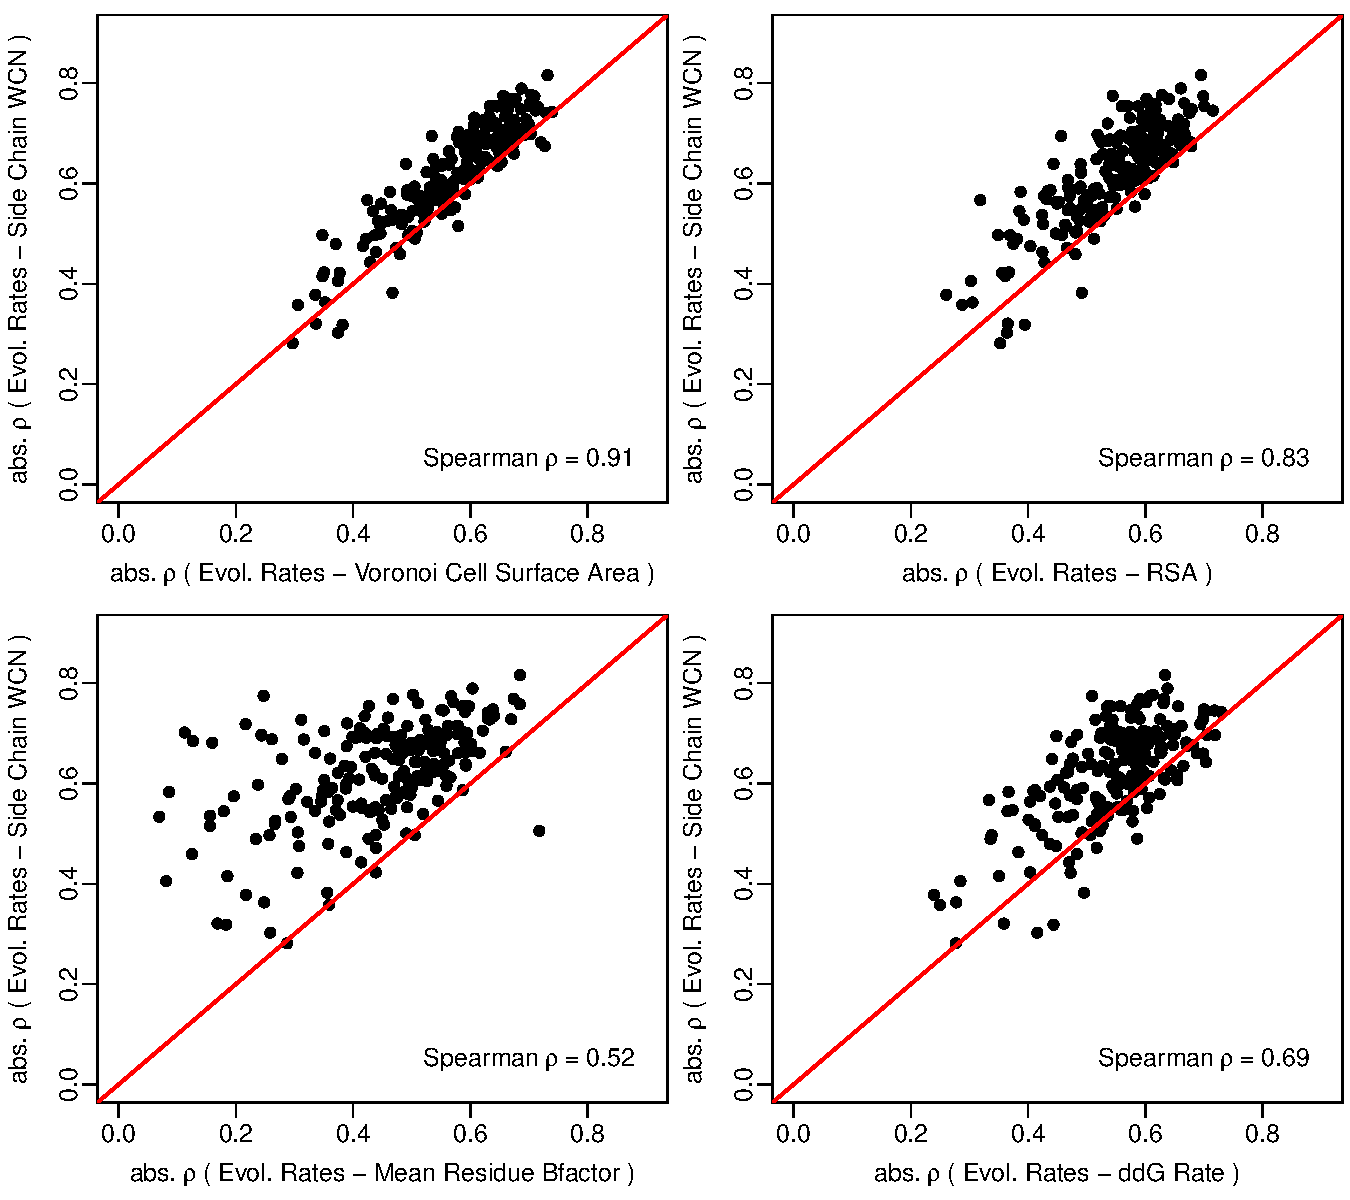
\includegraphics[width=6.9in]{cordiv_similarities_r4sJC.pdf}
            \end{center}
            \caption{A comparison of the strength of Spearman correlation of sequence evolutionary rates (r4sJC) with {\it side chain} Weighted Contact Number vs. correlations of other structural properties with evolutionary rates. Detailed description of the structural properties is given in Section \label{sec:mam}. The red lines in each plot represent equality line. It is evident from all plots that for any given protein in dataset, the correlation strength of one structural property is a good proxy measure of the correlation strength of any other structural property with sequence variability measures. For brevity, correlations of structure-rate4site are not shown here but are available online, also in supplementary material.}
            \label{fig:seqent_structure_cors}
        \end{figure}

        \begin{figure}[tbh]
            \begin{center}
            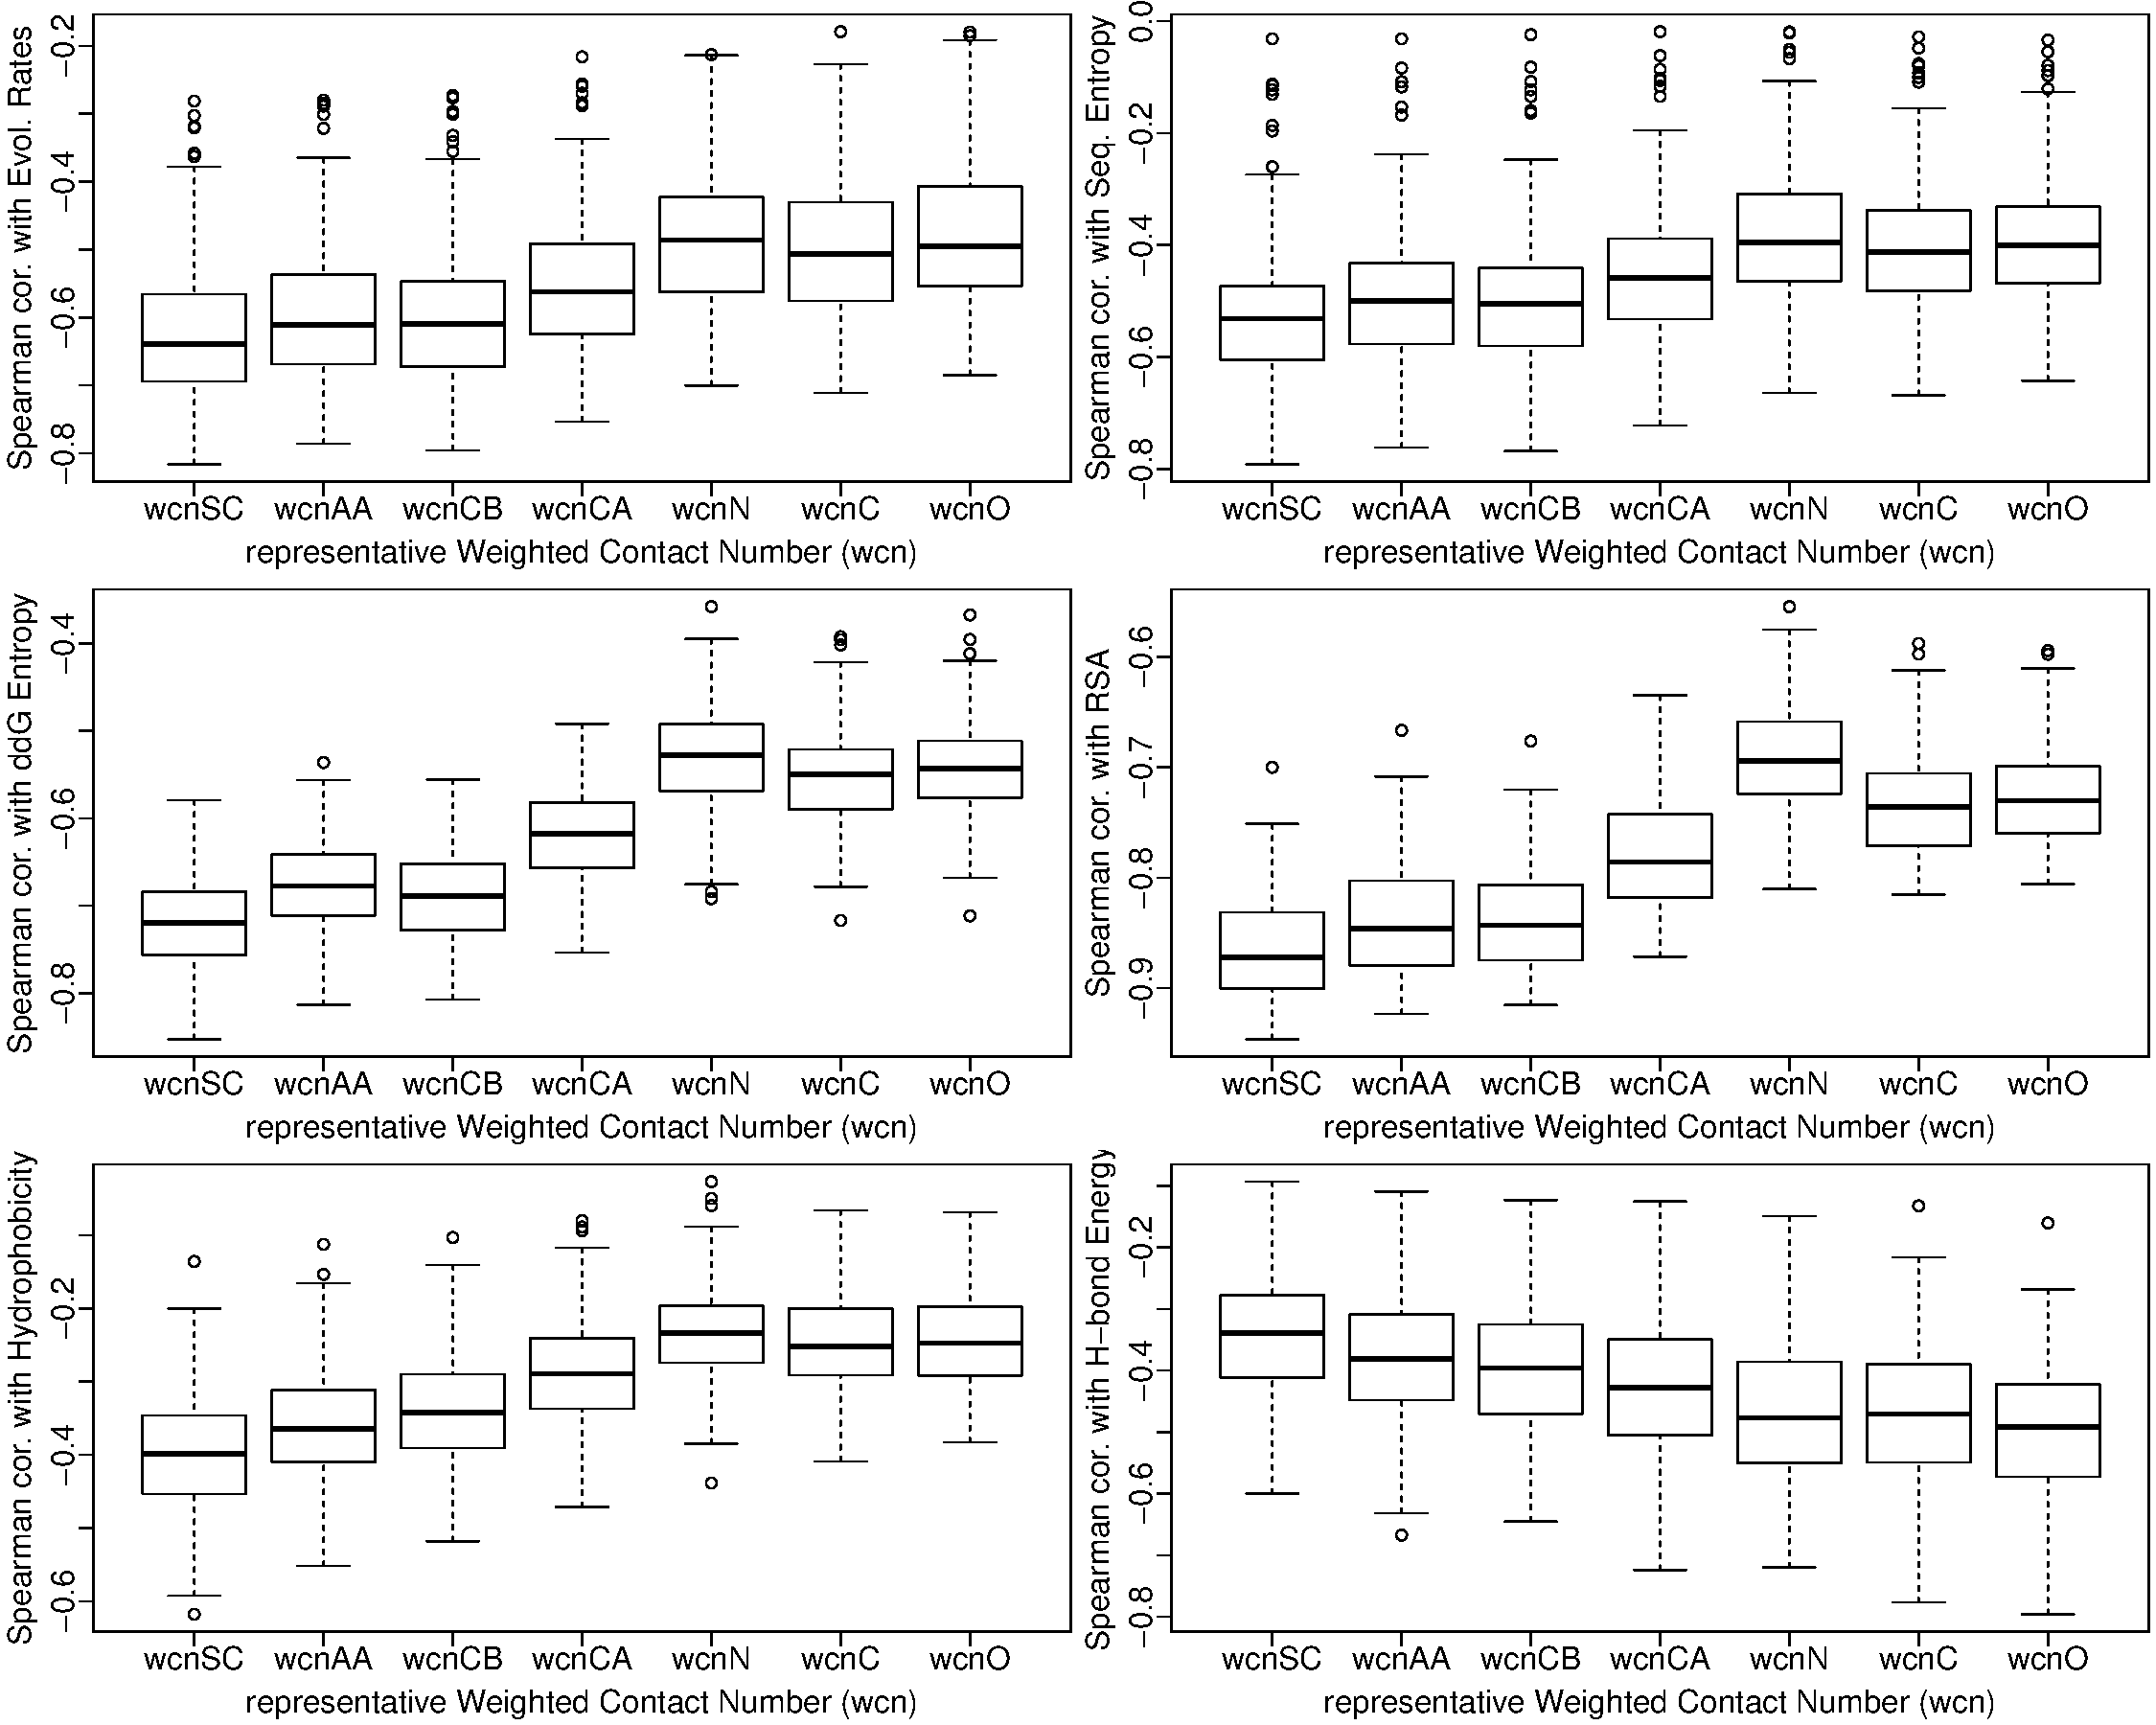
\includegraphics[width=6.9in]{/best_wcn/selected_variables/boxplot_wcn_all_in_one.pdf}
            \end{center}
            \caption{A comparison of the predictive power of different measures of Weighted Contact Number (WCN) about different structure or sequence properties for 209 proteins in dataset. In each plot, the Spearman correlation strengths of a given structure or sequence property on the vertical axis with different measures of WCN on the horizontal axis are compared against each other. The capital letters in the variable names on the horizontal axis denote the set of atomic coordinates used to calculate WCN. The variable $wcnSC$ denotes WCN measure based on the average coordinates over all heavy atoms in the side chain and the variable $wcnAA$ denotes WCN measure based on the average coordinate over all heavy atoms in the side chain and backbone of the amino acid.}
            \label{fig:best_wcn}
        \end{figure}

        \begin{figure}[tbh]
            \begin{center}
            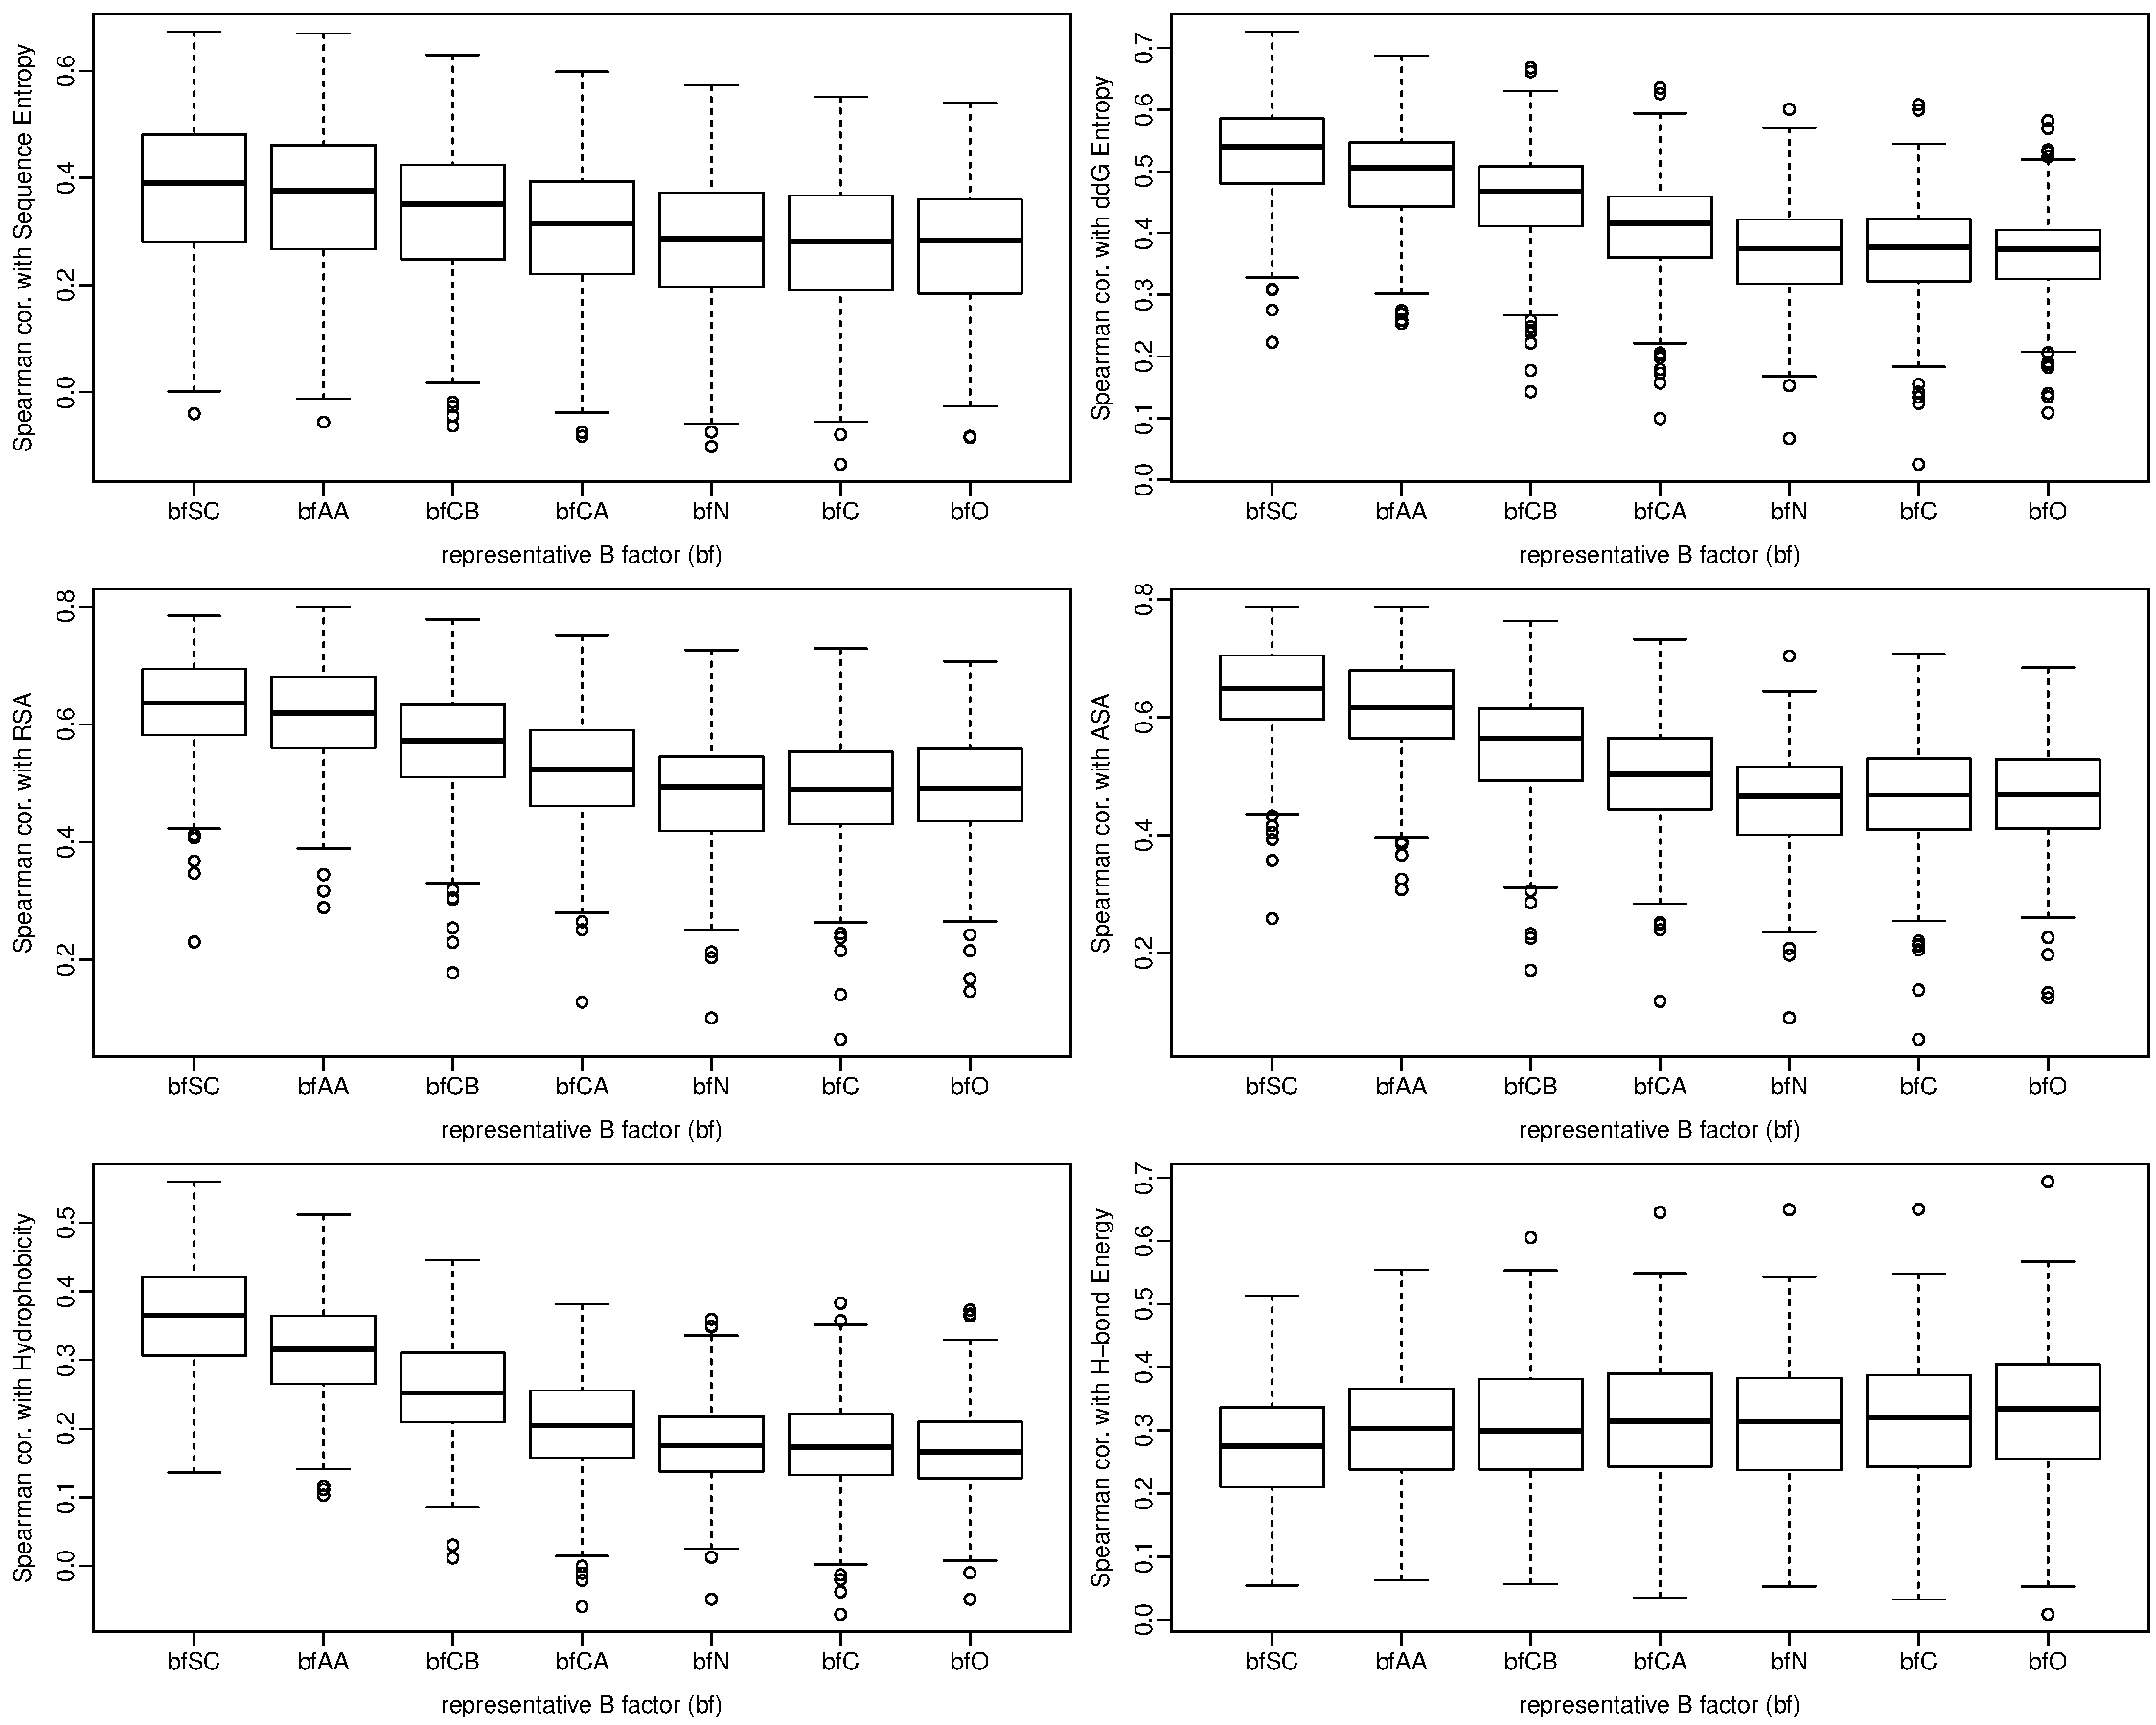
\includegraphics[width=6.9in]{/best_bf/selected_variables/boxplot_bf_all_in_one.pdf}
            \end{center}
            \caption{A comparison of the predictive power of different measures of Bfactor (BF) with different structure or sequence properties for 209 proteins in dataset. In each plot, the Spearman correlation strengths of a given structure or sequence property on the vertical axis with different measures of atomic Bfactors on the horizontal axis are compared against each other. The capital letters in the variable names on the horizontal axis denote the representative atomic Bfactors. The variable $bfSC$ denotes the average coordinate over all heavy atoms in the side chain for each site in protein and the variable $bfAA$ denotes average coordinate over all heavy atoms in the side chain and backbone of the amino acid.}
            \label{fig:best_bf}
        \end{figure}

        \begin{figure}[tbh]
            \begin{center}
            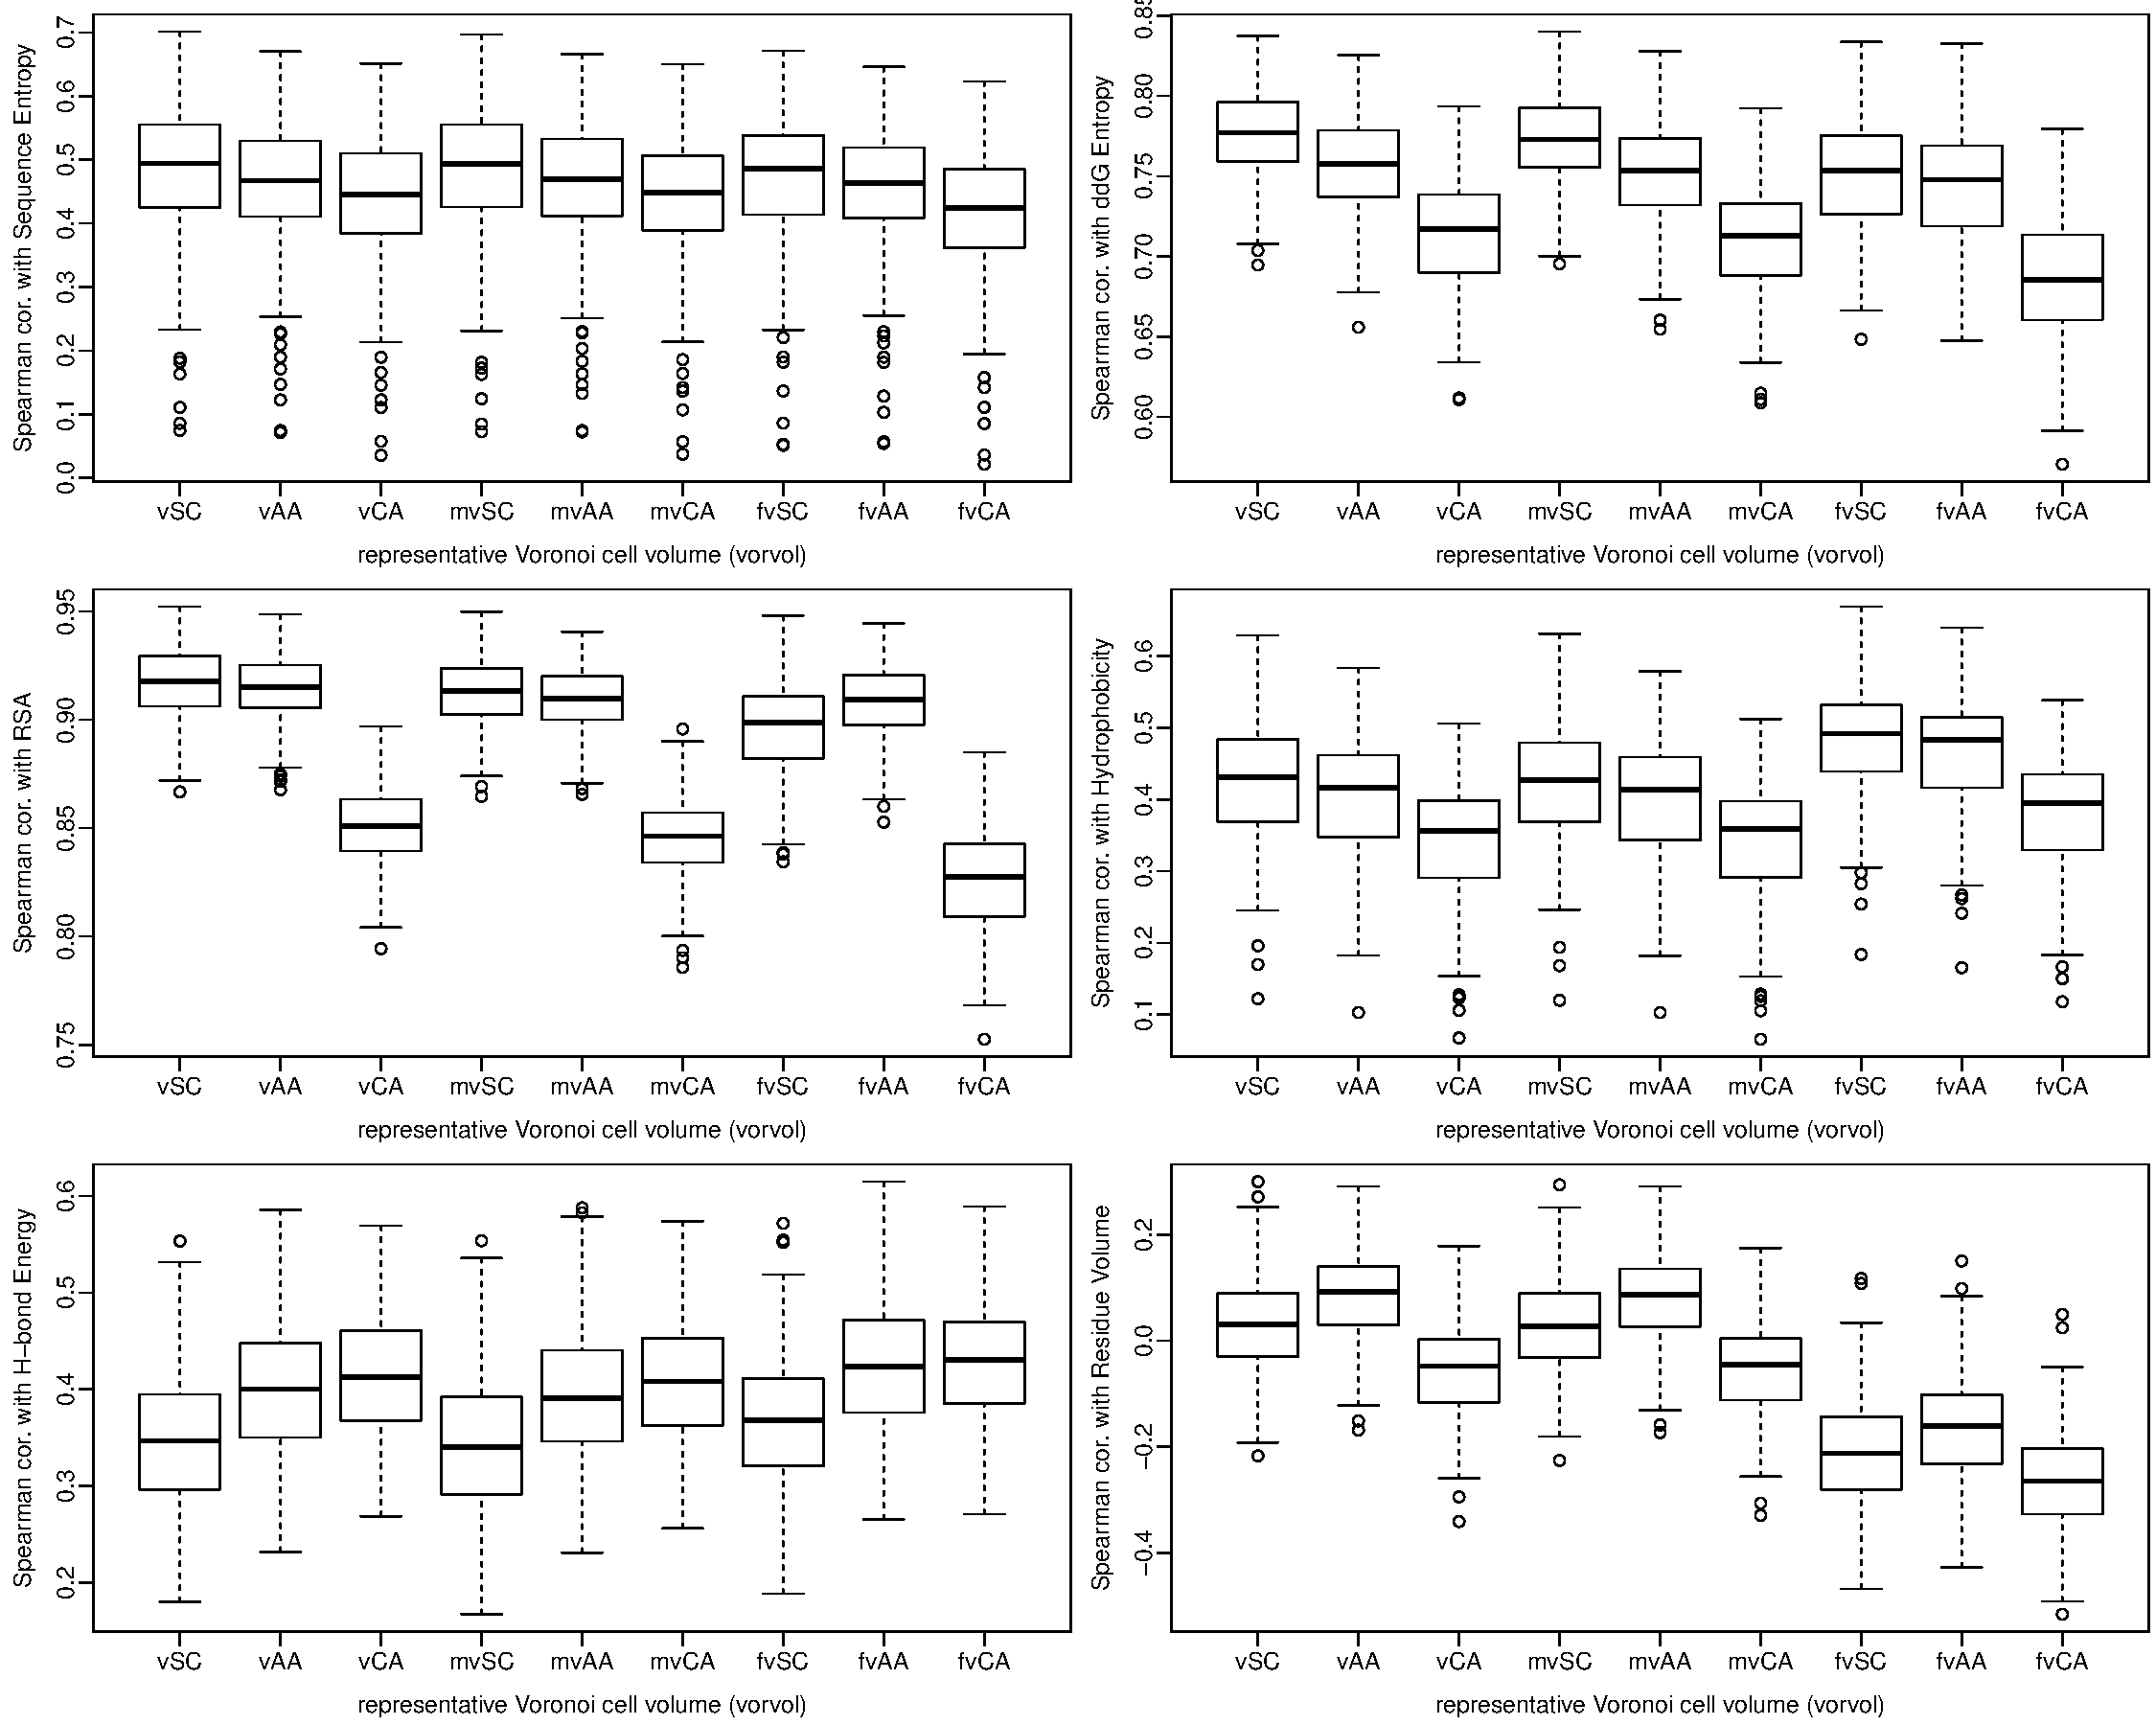
\includegraphics[width=6.9in]{/best_vorvol/selected_variables/boxplot_vorvol_all_in_one.pdf}
            \end{center}
            \caption{Should be likely modified to volume-area-length-sphericity measures instead.}
            \label{fig:best_voronoi}
        \end{figure}

        \begin{figure}[tbh]
            \centering
            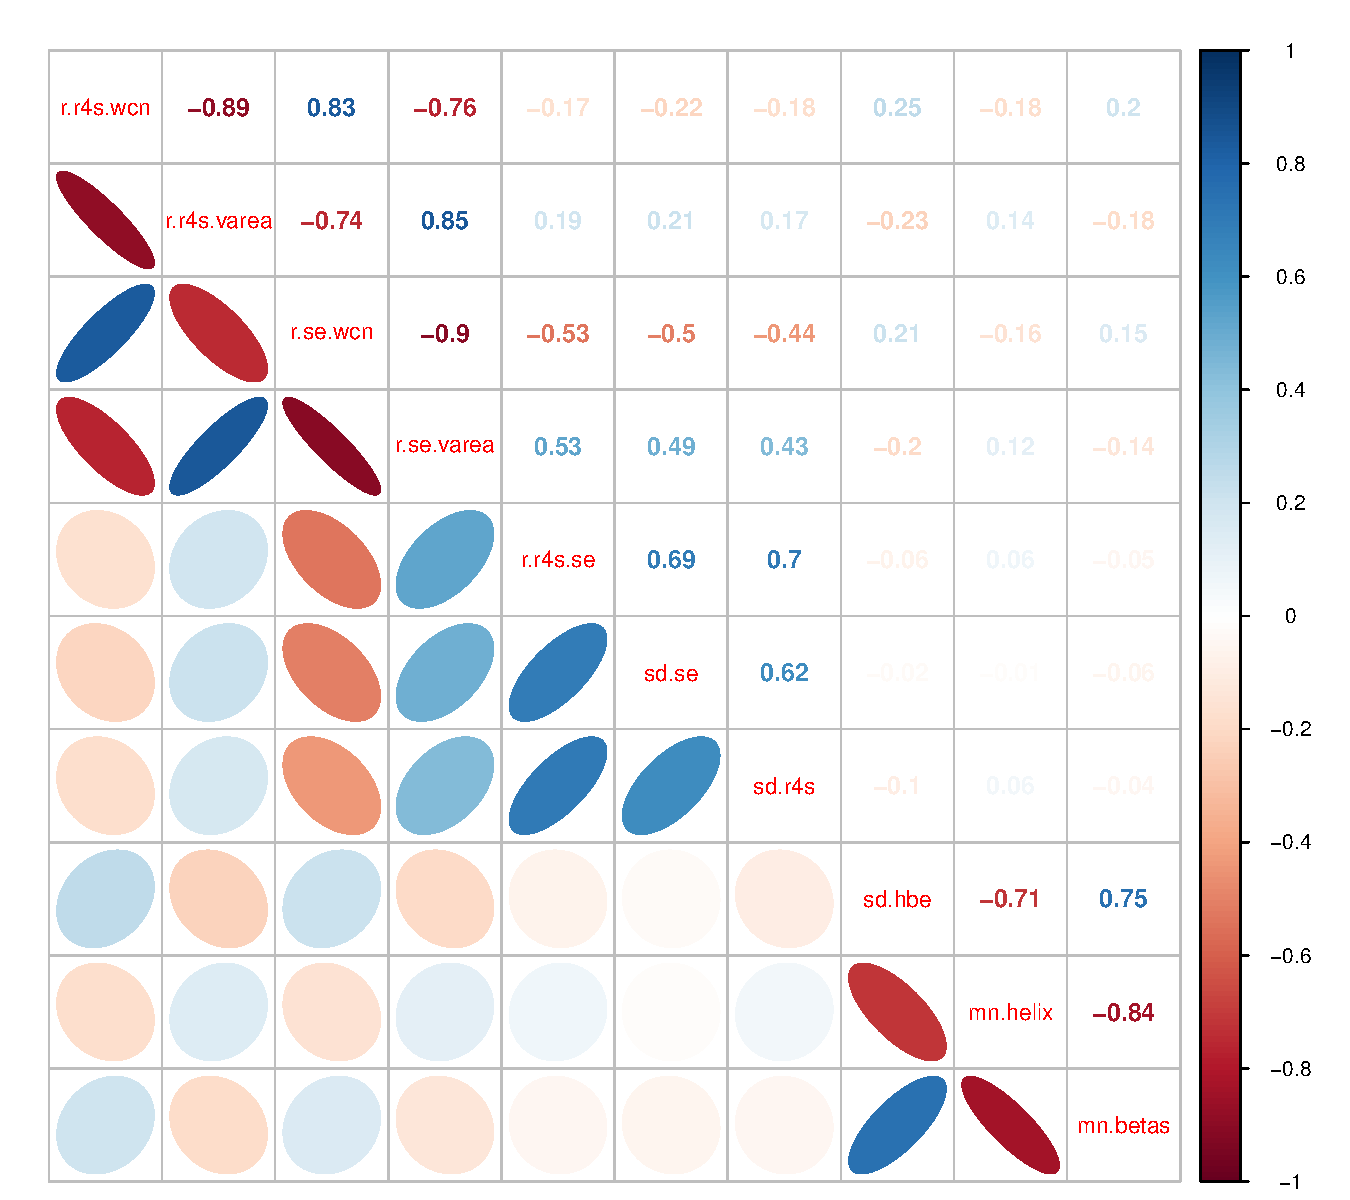
\includegraphics[width=7.2in]{/main_modulators_cormat.pdf} \\
            \caption{{\bf The Spearman correlation matrix of the strongest sequence--structure correlations and the prominent determinants of the strengths of the corresponding relations}. The variables on the diagonal elements of the matrix from top to bottom represent respectively, the four strongest sequence--structure relations: r4sJC--wcnSC, r4sJC--varea, seqent--wcnSC, seqent--varea, followed by protein properties that modulate the strength of these relations: the correlation between r4sJC--seqent ({\it r.r4sJC.seqent}), variance of r4sJC ({\it var.r4sJC}), variance of sequence entropy ({\it var.seqent}), the variance of hydrogen bond energies ({\it var.hbe}), and the fraction of helical \& $\beta-$sheet secondary structures in the proteins ({\it mean.helix} \& {\it mean.betas} respectively).}
            \label{fig:mainmods}
        \end{figure}

        \begin{figure*}[tbh]
            \centering
            \begin{tabular}{cc}
            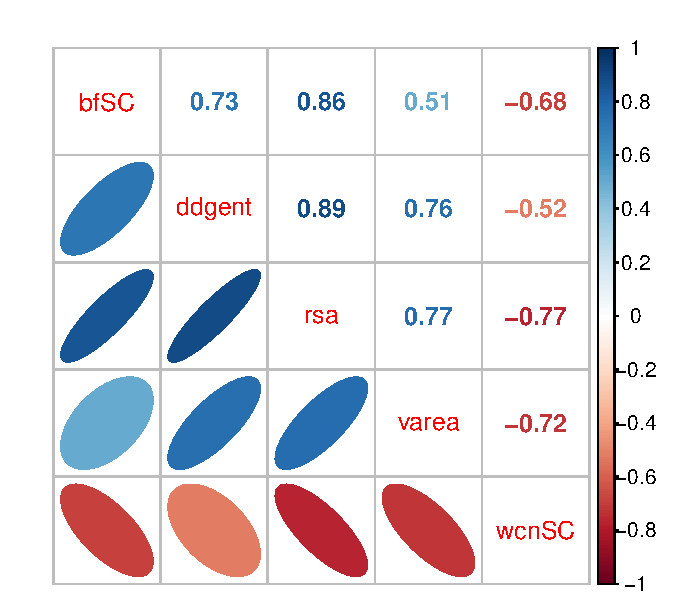
\includegraphics[width=3.4in]{/modulators_similarity_Sr4sJC_scors.pdf} & 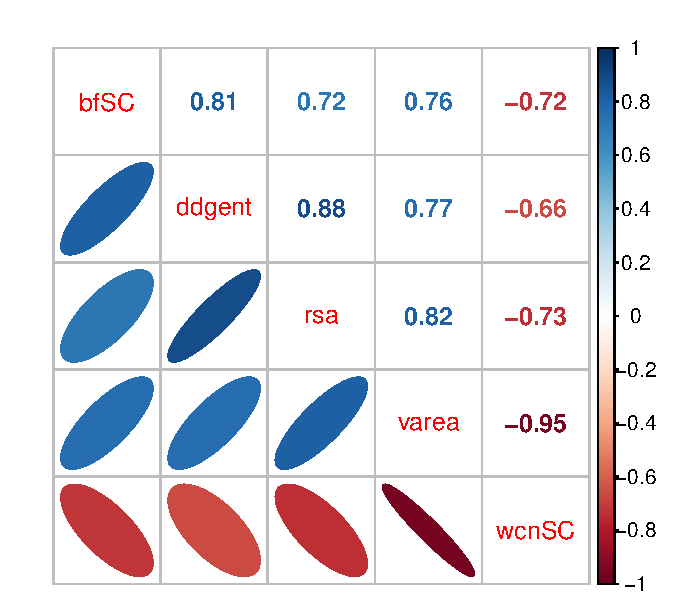
\includegraphics[width=3.4in]{/modulators_similarity_Sseqent_scors.pdf} \\
            \end{tabular}
            \caption{Proportion of explained variance of structure-sequence correlations by 182 pdb-level properties considered individually.}
            \label{fig:modsim}
        \end{figure*}

        \begin{figure*}[tbh]
            \centering
            \begin{tabular}{cc}
            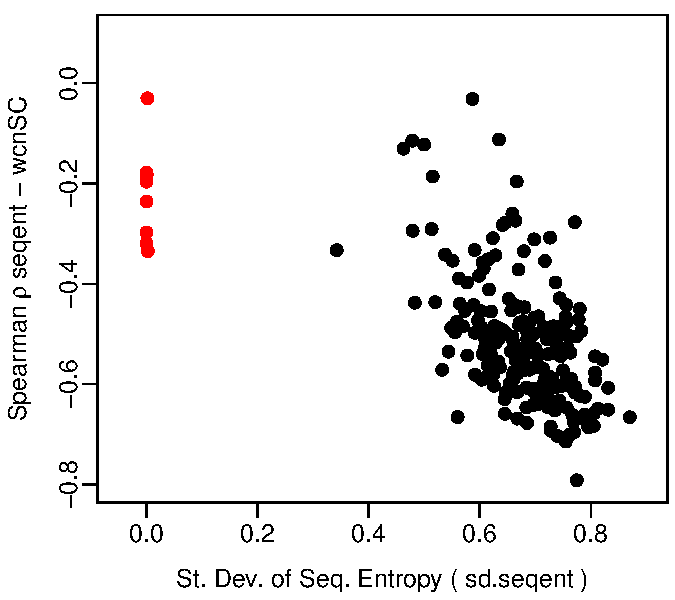
\includegraphics[width=3.4in]{/validation_sdseqent.pdf} & 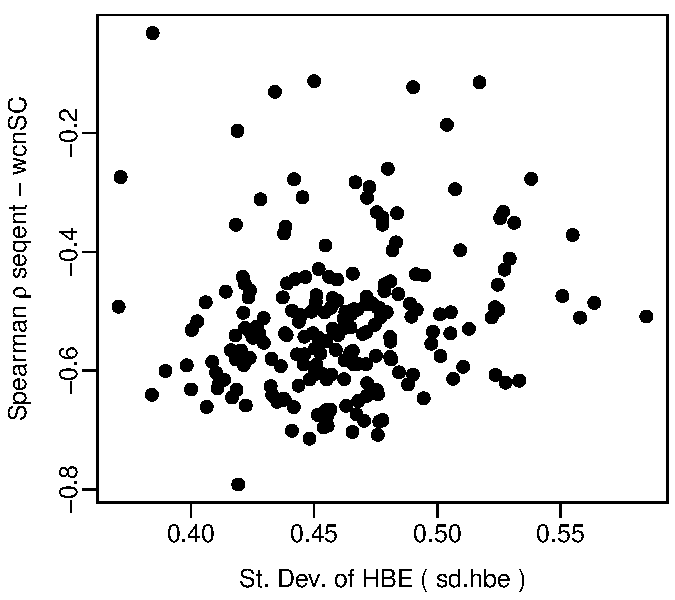
\includegraphics[width=3.4in]{/validation_sdhbe.pdf} \\
            \end{tabular}
            \caption{Proportion of explained variance of structure-sequence correlations by 182 pdb-level properties considered individually.}
            \label{fig:validation}
        \end{figure*}

\bibliographystyle{apj}
\bibliography{proc}

\end{document}

